% 五页作品介绍；由用户逐章确认的内容归并整理。使用 XeLaTeX 编译。
% 完整章节素材保留于本目录 01--07 文件；最终图表数据见第六章及文末证据索引。
\documentclass[UTF8,zihao=5,fontset=windows,a4paper]{ctexart}
\usepackage[left=20mm,right=20mm,top=18mm,bottom=18mm,headheight=14pt,headsep=5mm,footskip=9mm]{geometry}
\usepackage{amsmath,amssymb,booktabs,tabularx,array,graphicx,xcolor,fancyhdr,tikz,caption,hyperref}
\usetikzlibrary{arrows.meta,positioning,shapes.geometric}
\definecolor{ink}{HTML}{17384A}
\definecolor{accent}{HTML}{226C82}
\definecolor{muted}{HTML}{536570}
\hypersetup{unicode=true,colorlinks=true,linkcolor=accent,urlcolor=accent,
 pdftitle={面向线性PCurve的一类通用样条面到二次曲面智能转化方案},
 pdfsubject={基于线性PCurve的解析母面恢复、有限边界重建与独立几何验收},pdfauthor={BSpline2Analytic 项目}}
\ctexset{section={format=\large\bfseries\color{ink},beforeskip=8pt,afterskip=4pt},
 subsection={format=\normalsize\bfseries\color{ink},beforeskip=5pt,afterskip=2pt}}
\setlength{\parindent}{2em}
\setlength{\parskip}{2pt}
\linespread{1.12}
\setlength{\abovedisplayskip}{5pt}
\setlength{\belowdisplayskip}{5pt}
\captionsetup{font=small,labelfont=bf,skip=4pt,hypcap=false}
\pagestyle{fancy}\fancyhf{}
\fancyhead[L]{\small\color{muted}BSpline2Analytic\quad 作品介绍}
\fancyhead[R]{\small\color{muted}线性 PCurve · 有限面片解析化}
\fancyfoot[C]{\small\thepage\,/\,5}
\renewcommand{\headrulewidth}{0.3pt}
\fancypagestyle{first}{\fancyhf{}\fancyfoot[C]{\small\thepage\,/\,5}\renewcommand{\headrulewidth}{0pt}}
\newcommand{\key}[1]{\par\noindent\textbf{\color{ink}#1}\quad}
\newcommand{\note}[1]{{\small\color{muted}#1}}
\newcolumntype{Y}{>{\raggedright\arraybackslash}X}
\raggedbottom
\begin{document}
\thispagestyle{first}
\begin{center}
{\fontsize{19}{26}\selectfont\bfseries\color{ink}面向线性PCurve的一类通用样条面\par
到二次曲面智能转化方案\par}
\vspace{5pt}
{\small\color{muted}作品介绍\quad |\quad C++ / 海星 SGK 1.7.11\quad |\quad 2026 年 10 月}
\end{center}
\vspace{-6pt}
\section{项目背景}
在 CAD 模型交换与导入过程中，部分具有解析几何结构的曲面以非均匀有理 B 样条（NURBS）形式存储，可能来源于解析曲面的样条化转换、特定构型的圆角过渡或样条支撑曲面的裁剪。其形状仍可能在给定容差内符合解析曲面，而原有类型与几何参数未被显式保留。

恢复解析表示有助于减少控制顶点、节点及权重的存储开销，并为求交、投影和距离计算提供专用求解路径。但母面吻合并不足以保证有限面片转换有效，还需处理边界对应、参数化差异与退化。本项目据此构建识别、重建、必要优化和独立验收相衔接的自动转化方案。

\section{问题重述}
给定 NURBS 面片，判定其是否能够在容差内采用目标解析母面及有限边界表示；成功时恢复几何参数与边界，未完成可靠判定时返回可追溯状态。依据命题文件，评价目标如下；\textbf{命题目标与当前已验证能力分别陈述}。
\begin{center}\small
\renewcommand{\arraystretch}{1.14}
\begin{tabularx}{\linewidth}{@{}p{15mm}Y@{}}\toprule
目标 & 命题要求 \\\midrule
功能 & 完成样条面到目标解析曲面的可转换性判定与转换。\\
精度 & 曲面最大、平均距离及边界 Hausdorff 距离不超过 $10^{-5}\,\mathrm{mm}$；相邻面公共边界法向夹角不超过 $0.1^\circ$（命题的 G1 误差要求）。\\
性能 & 50--200 个控制顶点的单面片判定不超过 $10\,\mathrm{ms}$；转换后投影、求交和布尔运算耗时降低至少 $50\%$，须另行验证。\\
工程 & C++ / SGK 1.7；连续处理 1,000 个不同复杂度输入，无崩溃、内存泄漏或结果不一致，异常信息清晰可追溯。\\\bottomrule
\end{tabularx}
\end{center}

\section{条件假设及面向场景}
支持平面、圆柱面、圆锥面、球面，并将\textbf{规则圆环面作为扩展解析目标}。输入节点、次数及控制顶点有效，有理权重为正，内部节点连接无位置不连续。工程验证重点为不超过 200 个控制顶点；当前一般路径固定数据两方向次数为 3--5，该次数范围属于验证条件。

核心约束作用于\textbf{目标母面对应的 NURBS 参数域}。记其参数化为 $\mathbf Q:\Omega_Q\subset\mathbb R^2\to\mathbb R^3$，目标边界为
\[
\boldsymbol\ell_i(t)=(1-t)\mathbf a_i+t\mathbf b_i,\qquad
\widehat{\mathbf c}_i(t)=\mathbf Q(\boldsymbol\ell_i(t)),\quad t\in[0,1].
\]
线性 PCurve 不要求三维边界为直线，也不等于解析原生角度参数中的直线；源面与目标面的参数域需要区分。源、目标边界允许经调整方向后的连续单调参数对应比较。一般路径由四个源参数侧恢复单一凸四边形或满足退化判据的三角形；非线性 PCurve、多环和带孔裁剪不在承诺范围内。

位置容差保持 $10^{-5}\,\mathrm{mm}$。仅当源段、目标段的连续三维直径上界均不超过 $10^{-8}\,\mathrm{mm}$ 时允许微小分段切向豁免，仍验收位置并记录区间。一般兜底采用内部采样与连续边界认证，不代表全域连续内部距离或相邻面 G1 保证。以 $10\,\mathrm{ms}$ 评价性能，共享 $50\,\mathrm{ms}$ 总预算；超限即计算失败，不据此断言几何无解。

\newpage
\section{技术架构总览}
方案采用\textbf{统一调度、等参优先、一般兜底、独立验收}的架构。所有输入先经过等参专用分支，未获得有效结果时在剩余预算内进入一般分支。候选生成、参数优化与最终验收各负其责：优化改善候选，验收决定是否接受。

\begin{center}
\begin{tikzpicture}[node distance=4mm and 7mm,
 box/.style={draw=accent,rounded corners,align=center,font=\small,inner sep=4pt,text width=62mm},
 decision/.style={draw=accent,diamond,aspect=5,align=center,font=\small,inner sep=1pt},
 arr/.style={-{Stealth},semithick,draw=accent}]
\node[box] (in) {输入与选项检查、统一预算及结果管理};
\node[box,below=of in] (iso) {等参路径：有理识别 / 非有理候选搜索\\母面与边界验收；失败候选继续搜索};
\node[decision,below=of iso] (ok) {等参通过？};
\node[box,below=of ok] (pool) {一般路径：候选去重、渐进评分与分批选择};
\node[box,below=of pool] (val) {参数图与线性边界恢复 → 输出构造 → 验收};
\node[decision,below=of val] (pass) {通过？};
\node[box,below=of pass] (opt) {未通过且允许优化：改善母面参数后重验\\仍失败则取下一候选；耗尽则返回失败};
\node[box,text width=31mm,right=15mm of pool] (out) {返回前复核总耗时\\成功输出 / 失败诊断};
\draw[arr] (in)--(iso);\draw[arr] (iso)--(ok);
\draw[arr] (ok)--node[right,font=\small]{否}(pool);
\draw[arr] (pool)--(val);\draw[arr] (val)--(pass);
\draw[arr] (pass)--node[right,font=\small]{否}(opt);
\draw[arr] (ok.east)-|node[pos=.25,above,font=\small]{是}(out.north);
\draw[arr] (pass.east)-|node[pos=.25,above,font=\small]{是}(out.south);
\draw[arr] (opt.west)--++(-12mm,0)|-node[pos=.25,left,font=\small,align=center]{下一\\候选}(val.west);
\draw[arr] (opt.east)-|node[pos=.25,below,font=\scriptsize]{重验通过 / 耗尽}(out.south east);
\end{tikzpicture}
\captionof{figure}{总体与求解子流程。期限检查贯穿各阶段；预算耗尽统一返回失败。}
\end{center}

\key{统一调度与分析上下文}各分支分别建立分析上下文，在分支内按需复用求值、导数和采样数据。输入保持不变；候选单独构建，失败时清除可供下游使用的结果。等参子预算默认 20 ms，两分支共享从同一起点计算的 50 ms 总预算。

\key{等参识别与一般候选}有理输入进入相应识别路径，非有理输入执行增量等参候选搜索与验收。一般分支采用分离的生成与评价样本，按类型生成母面候选，经几何去重、评分后分批验证；失败候选按配置进行一轮母面参数优化，改善后重新验收。

\key{优化与边界恢复}优化以采样点到母面的投影残差为基础，按距离容差归一化，采用受约束的阻尼最小二乘 / 信赖域迭代；一般母面 Jacobian 采用差分构造。目标是改善母面参数，不替代验收。边界模块恢复参数图、端点和直线连接，处理周期接缝与退化，构造共享端点的三维 NURBS 曲线。

\begin{center}\small\renewcommand{\arraystretch}{1.18}
\begin{tabularx}{\linewidth}{@{}p{28mm}Y@{}}\toprule
验收路径 & 实际验收范围 \\\midrule
有理等参识别 & 相应的母面、参数范围与边界检查；保留识别报告中的 Bernstein 界。\\
非有理等参路径 & 带浮点保护的全域母面距离界、四边位置对应及同区间 U/V 切向联合预算；不构造相邻面 G1 证书。\\
一般兜底 & 内部及有限面片采样距离、实际输出边界连续位置与沿边切向认证；显式记录切向不适用及豁免范围。\\\bottomrule
\end{tabularx}
\end{center}
\noindent\note{求界子流程：分段与对应建立 → 误差包络快速判定 → 区间重算 → 必要时细分并重建对应 → 接受、未认证或预算失败。不同路径保留各自验收范围。}

\newpage
\section{创新点介绍}
本方案的创新重点是面向线性 PCurve 有限面片的建模、求解及验收协同设计。以下概括八个相互衔接的技术主题，强调已有数值工具在本问题中的组合与实现。

\key{1. 统一边界模型与齐次直接构造}在目标 NURBS 参数域中统一描述等参和斜向直线边界。若 $\mathbf Q=\mathbf P/w$，则沿线性 PCurve 的边界为 $\widehat{\mathbf c}(t)=\mathbf P(\boldsymbol\ell(t))/w(\boldsymbol\ell(t))$。在 Bernstein 基下进行代数复合，跨单元时按交点分段，使边界结构直接参与输出生成；浮点系数转换与拼接误差另行验收。

\key{2. 结构驱动搜索与具有下界依据的渐进评分}等参分支优先利用明确结构，一般分支补充多类型候选。评价子集上的最大距离是完整评价集最大距离的下界，因而可按当前批次阈值延后不具竞争力候选的完整求值，后续批次仍可继续处理。部分均方根误差不具有同样性质，不用于该判定；评分始终不替代最终验收。

\key{3. 圆环面轴线候选的几何恢复}由四组位置与法向建立轴线约束，以方向和矩表示直线 $\mathbf L=(\mathbf d,\mathbf m)$。带列主元 QR 求得零空间后，利用 $\mathbf d\!\cdot\!\mathbf m=0$ 的二次关系枚举候选轴线，再通过条件化子午圆拟合恢复中心及主、次半径。多解进入后续评分，避免过早固定不确定的轴向。

\key{4. 将数值可辨识性纳入初始化}局部平移与尺度归一化减轻大坐标量级影响；奇异值比例、方向分离度和构造残差用于识别秩亏、轴向歧义。直接对原始矩阵分解，避免法方程的条件数平方效应；结合分布较广的多点支撑与多组初始化，不依赖单次局部采样确定全部参数。

\key{5. 参数图与边界对应协同恢复}对于球面，在保持球心和半径不变的条件下提出有限数量的坐标框架；周期方向按整周期平移保持边界连接一致。验收细分可依据源几何位置更新目标参数分割点，并重建局部误差及切向残差，使认证始终对应当前映射。有限候选搜索不解释为对所有参数化的穷尽。

\key{6. 正比例切向残差的连续角度验收}在同一局部参数区间内，以切向量或有理切向分子 $\mathbf A,\mathbf B$ 构造 $\mathbf R=\mathbf A-\lambda\mathbf B$，其中 $\lambda$ 连续为正。若有正的长度下界且
\[
\eta=\frac{\sup\|\mathbf R\|}{\inf\|\mathbf A\|}<1,
\qquad \text{则 }\mathbf A\cdot\mathbf B>0,\quad\sin\angle(\mathbf A,\mathbf B)\le\eta.
\]
这一构造分离方向差异与参数速度差异，避免构造切向样条叉乘。数值选取的缩放函数仅用于提出残差，最终接受依赖保守求界；界不充分时细分或报告未认证，不直接断言真实角度超限。

\key{7. 实际输出验收与自适应认证开销}输出完成次数统一、权重处理及共享端点设置后，从内核对象重新读取系数，检查实际曲线与理想母面轨迹的偏差，并验收源边界到实际输出的误差。认证采用保守浮点包络、区间重算与细分分层执行，按判定收益关闭重复快速计算，复用组合系数与位置误差界；加速不改变接受阈值。

\key{8. 有覆盖依据的退化处理与预算失败语义}依据连续三维直径界处理微小分段，保留完整位置覆盖并记录切向豁免。整边坍缩、极点与锥顶分别按适用条件处理。结果记录实际路径、候选数、迭代数、验收与超时阶段，区分误差见证、未认证及预算退出；超时结果不得作为有效转换输出。

\par\vspace{4pt}\noindent\note{这些机制共同将母面参数、有限边界和实际内核对象纳入同一验证链条。效率收益与成功范围以可复现测试为依据，不由方法名称推定。}

\newpage
\section{应用场景结果展示}
选取球面极点、圆锥顶点和规则圆环面三角形裁剪三个案例。前两例来自固定数据，后一例为本次补充的可复现正例。所有调用均先进入等参分支，未通过后进入一般兜底；算法不接收来源母面或预设参数图。

Windows x64 / MSVC Release 下，每例串行重复三次、新建算法上下文，无逐例预热，保留首次调用。\textbf{整体耗时覆盖统一 API 调用至返回}，排除加载、来源认证、输出审计、绘图及文件写入；取三次最大值严格判断是否小于 10 ms，超过 50 ms 强制失败。未独占机器或固定 CPU 亲和性。

\begin{center}\small\renewcommand{\arraystretch}{1.22}
\begin{tabularx}{\linewidth}{@{}Yccccc@{}}\toprule
案例 & 成功且审计通过 & 边界上界/mm & 最大/ms & $<10$ ms & $\le50$ ms\\\midrule
球面 case-317 & 3/3 & $4.14\!\times\!10^{-7}$ & 6.9672 & 是 & 是\\
锥顶 case-217 & 3/3 & $5.23\!\times\!10^{-7}$ & 2.7237 & 是 & 是\\
圆环 torus-triangle & 3/3 & $2.72\!\times\!10^{-11}$ & 2.3761 & 是 & 是\\\bottomrule
\end{tabularx}
\end{center}
\noindent\note{边界距离为连续认证上界，向上取整展示，均小于 $10^{-5}\,\mathrm{mm}$。三例均有一条整边坍缩，微小分段切向豁免数、母面优化迭代数均为零。}

\subsection*{（1）球面极点：参数退化下的边界恢复}
双五次非有理样条、64 个控制顶点，一条参数边坍缩至球面极点。球面在该点保持几何正则，退化发生于当前参数化。输出恢复母面与有限边界，保留坍缩边位置验收，对其余边界执行连续切向检查。
\begin{center}
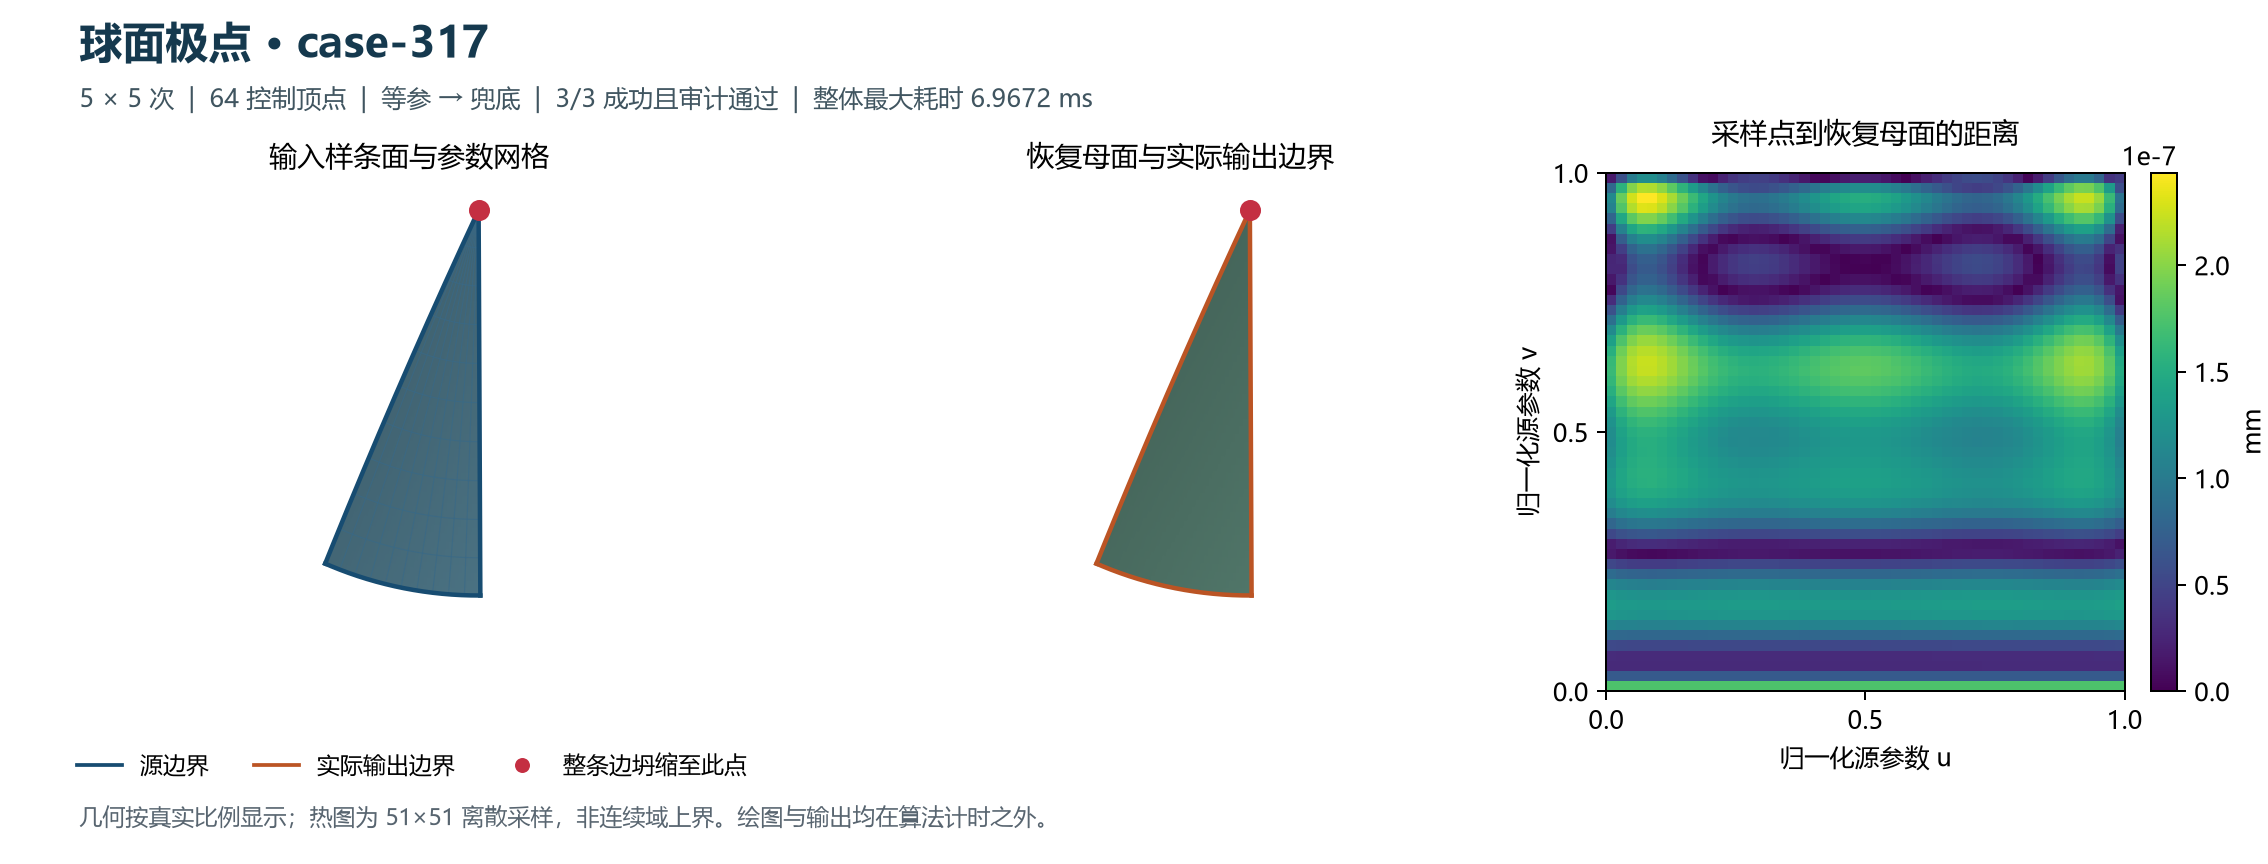
\includegraphics[width=\linewidth]{figures/sphere-317.png}
\captionof{figure}{球面极点：实际输入、恢复母面与输出边界、采样距离分布。}
\end{center}

\subsection*{（2）圆锥顶点：几何奇点处的位置保持}
五次／三次非有理样条、64 个控制顶点，一条参数边整体收缩至几何奇点锥顶。转换保留顶点位置与相邻边界连接，非退化边界继续验收位置和切向；独立审计检查实际曲线的共享端点与边界距离。
\begin{center}
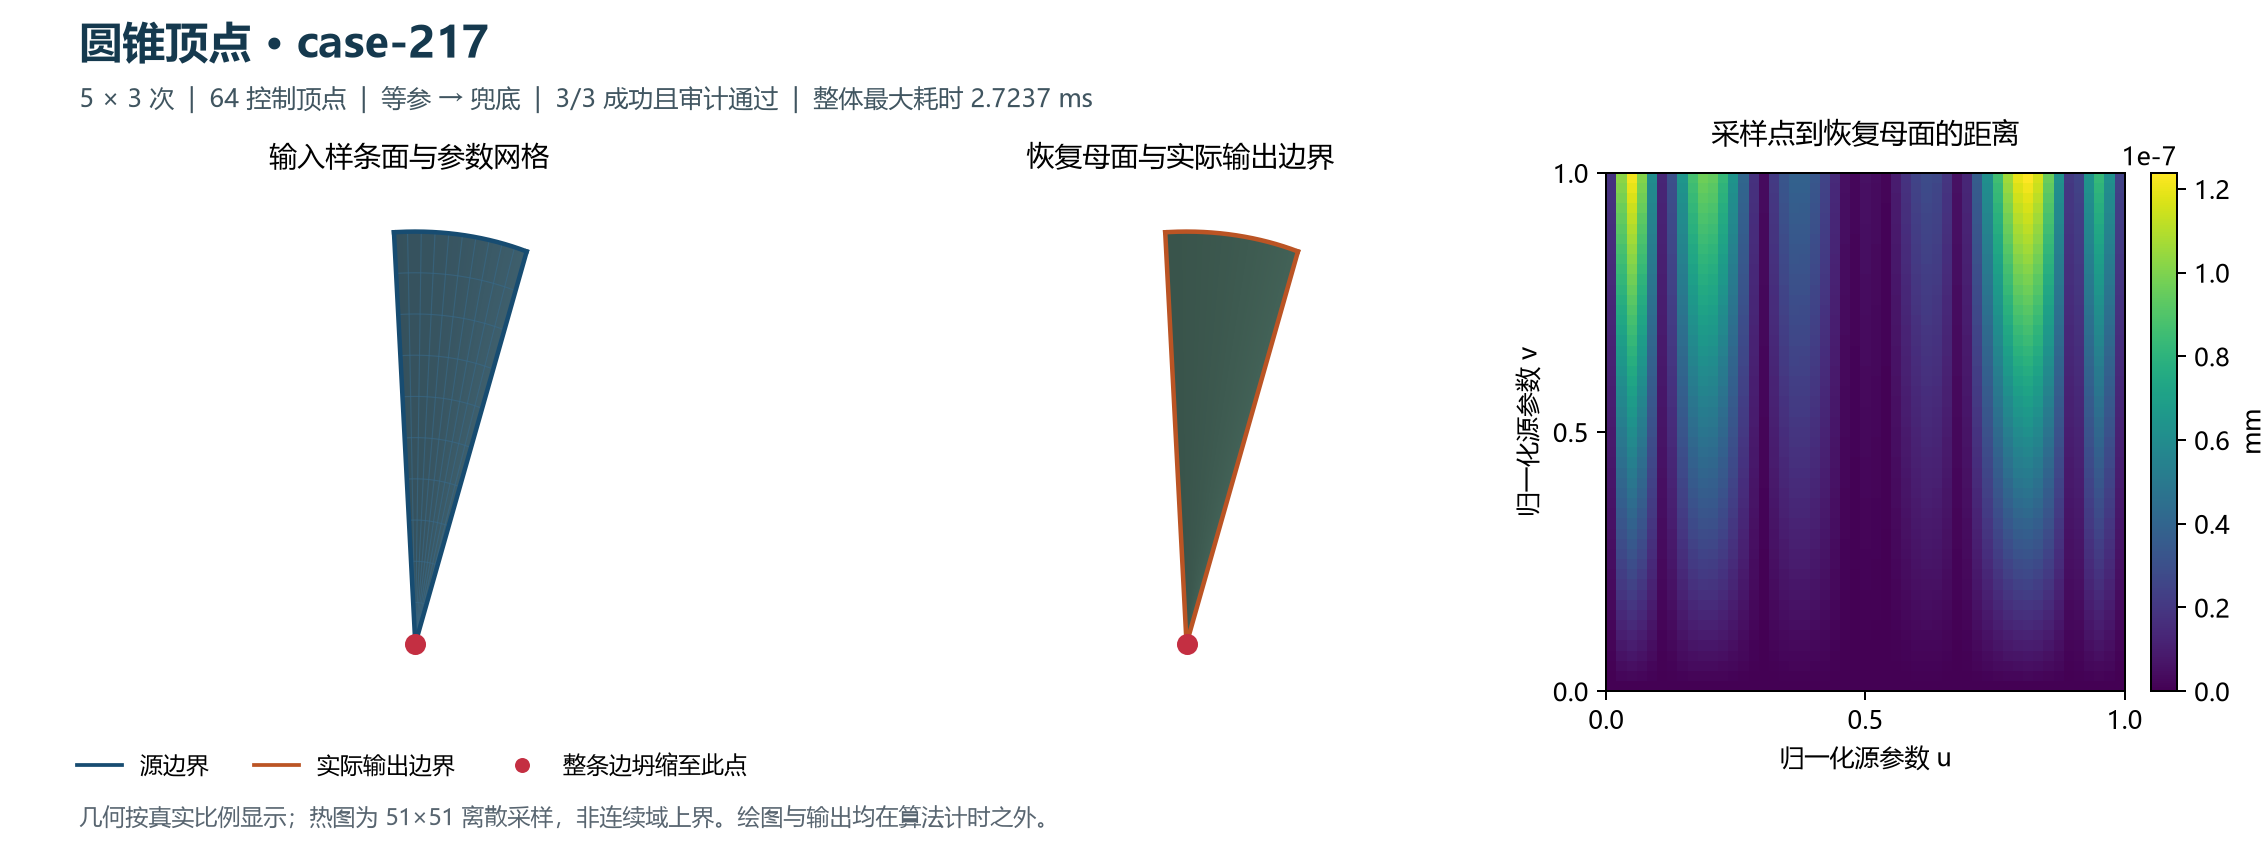
\includegraphics[width=\linewidth]{figures/cone-217.png}
\captionof{figure}{圆锥顶点：整边坍缩被显式处理，未通过放宽位置容差接受结果。}
\end{center}

\newpage
\subsection*{（3）圆环面坍缩边：正则母面上的三角形裁剪}
三次／四次有理样条、63 个控制顶点。采用固定数据 main-400 的规则圆环母面参数，通过独立来源生成器构造三角形裁剪正例，源参数边 $V_{\max}$ 映射到同一点。\textbf{退化的是面片参数边，圆环母面本身保持正则。}算法独立恢复母面、参数区域与三维边界，无需为保持四边结构人为保留短边。
\begin{center}
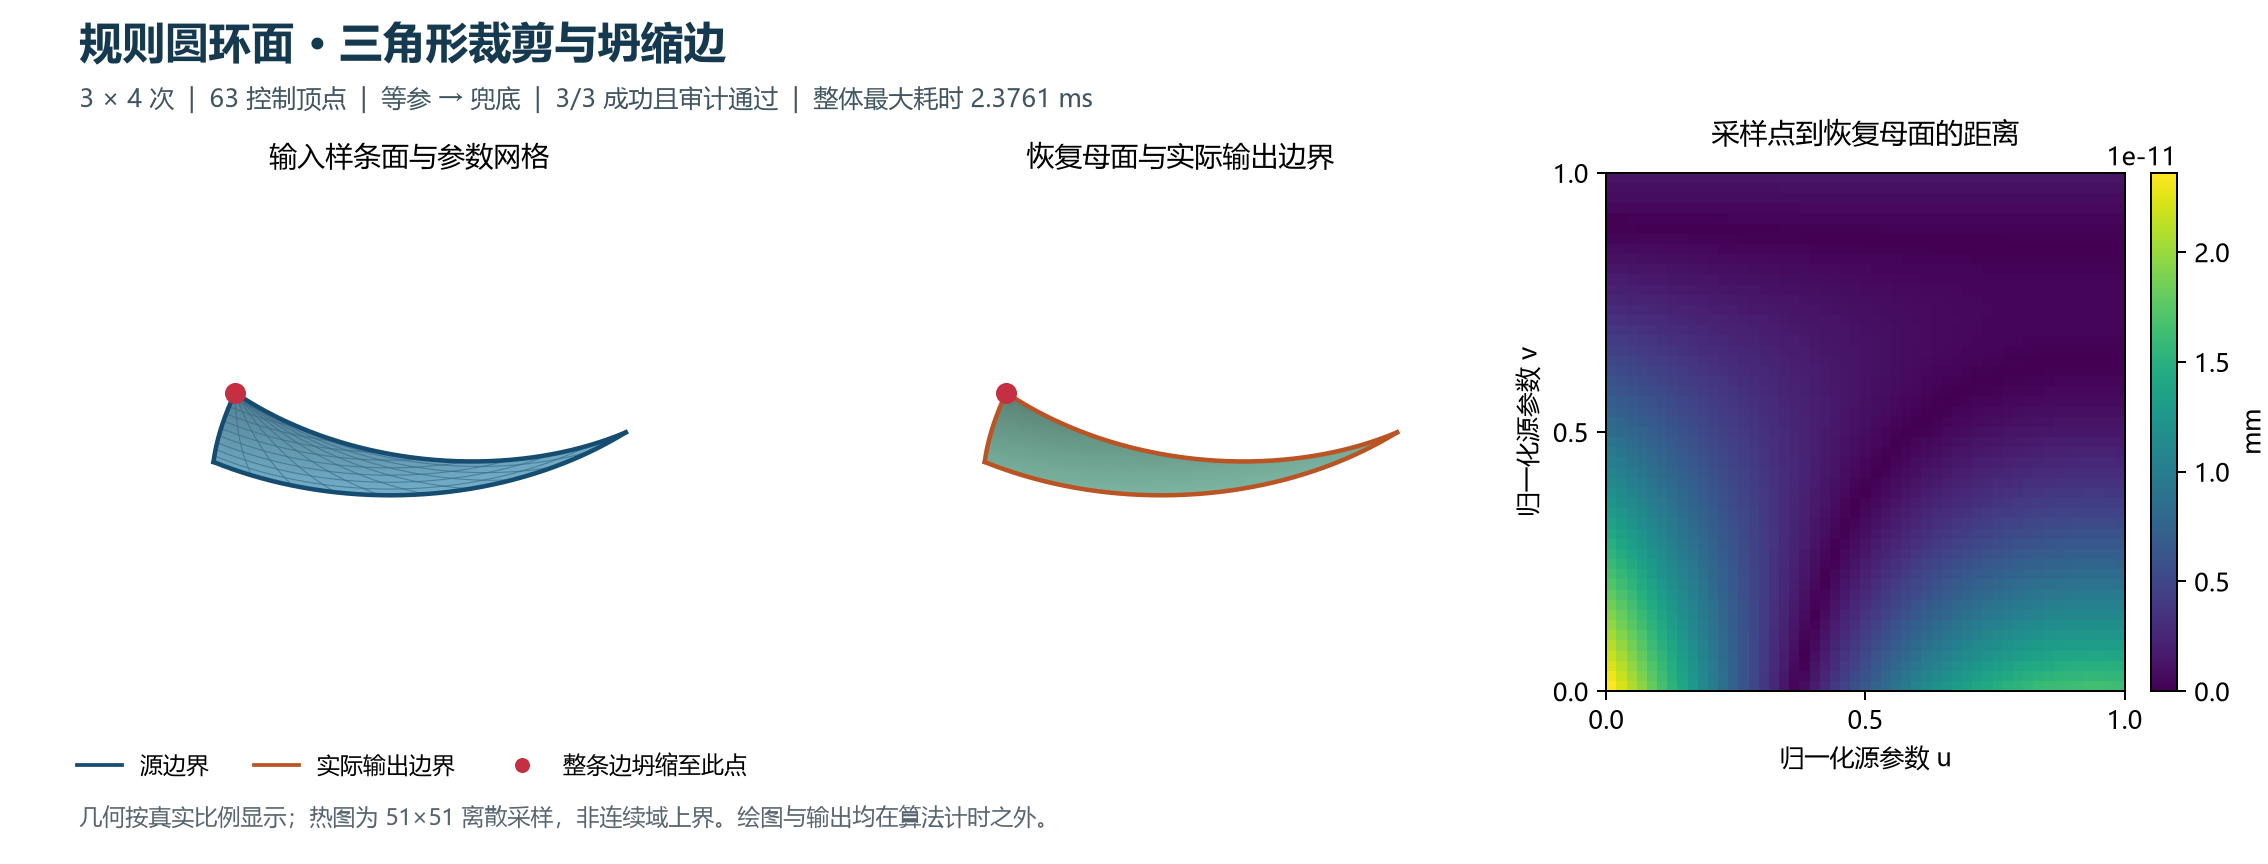
\includegraphics[width=\linewidth]{figures/torus-triangle.png}
\captionof{figure}{圆环面三角形裁剪：源参数网格汇聚于坍缩点，输出保持有限边界。}
\end{center}

三图左侧为实际输入求值，中间为恢复母面及参数区域的显示网格与\textbf{实际内核输出边界}，并非已构造的拓扑面。红点标记整边坍缩位置。左右采用同一局部正交坐标系、相机及等比例缩放，不放大几何误差；热图为 $51\times51$ 源采样点到恢复母面的距离，各图独立色标，不能视为全域上界。

三个案例的非坍缩边界切向上界分别约为 $0.001072^\circ$、$0.001361^\circ$ 和 $2.555\times10^{-9}\,{}^\circ$。坍缩边的切向不适用，不能记作零角度认证。上述定向测试验证分支衔接、边界恢复与退化处理，不作为优化器效果证据，也不替代全量回归。

\section{总结}
本作品以目标母面 NURBS 参数域中的线性 PCurve 为边界约束，将解析母面识别、参数恢复、有限边界重建及独立几何验收纳入统一流程，为导入模型的表示简化和后续解析运算提供基础。

主要贡献是\textbf{结构驱动求解与可追溯验收的结合}：等参优先与一般候选搜索兼顾效率和适用范围；齐次复合将边界约束落实为有理几何；正比例切向残差及分层求界提供连续验收依据；实际输出复核连接数学构造与内核表示。对极点、锥顶、坍缩边和预算退出作显式处理，使成功与失败均具有明确解释。

三个代表案例均通过转换与独立输出审计，各例三次测试的最大整体耗时均小于 10 ms，展示了方案在有限面片恢复与退化边界处理中的实际能力。作品形成了具有明确适用条件、独立验收机制和可复现测试依据的工程实现，为 CAD 几何内核中的解析几何恢复提供了可集成的算法基础。

\begin{center}\small\renewcommand{\arraystretch}{1.17}
\begin{tabularx}{\linewidth}{@{}p{30mm}Y@{}}\toprule
核对项 & 当前结论与证据边界\\\midrule
已实现 & 等参优先、失败兜底、线性边界恢复、实际输出验收、共享预算与诊断。\\
已展示 & 三个定向正例共 9 次成功且审计通过；全部 $<10$ ms、$\le50$ ms；零优化迭代。\\
\bottomrule
\end{tabularx}
\end{center}

\noindent\note{\textbf{证据索引（仓库内）}\par
命题：\path{docs/requirements/} 下“中船海舟样条转二次曲面.pdf”。\par
定向结果：\path{docs/testing/introduction-cases-2026-10-16/} 的 \path{runs.csv}、\path{summary.json}、\path{provenance.json}；证据提交 \texttt{a32b2a9}，源码及输入哈希见 provenance。\par
历史全量批次：\path{docs/testing/SEQUENTIAL_NON_EXTREME_2026-10-16.md}。\par
运行器：\path{tests/IntroductionCases.cpp}。}
\end{document}
